\documentclass[twoside]{book}

% Packages required by doxygen
\usepackage{fixltx2e}
\usepackage{calc}
\usepackage{doxygen}
\usepackage[export]{adjustbox} % also loads graphicx
\usepackage{graphicx}
\usepackage[utf8]{inputenc}
\usepackage{makeidx}
\usepackage{multicol}
\usepackage{multirow}
\PassOptionsToPackage{warn}{textcomp}
\usepackage{textcomp}
\usepackage[nointegrals]{wasysym}
\usepackage[table]{xcolor}

% Font selection
\usepackage[T1]{fontenc}
\usepackage[scaled=.90]{helvet}
\usepackage{courier}
\usepackage{amssymb}
\usepackage{sectsty}
\renewcommand{\familydefault}{\sfdefault}
\allsectionsfont{%
  \fontseries{bc}\selectfont%
  \color{darkgray}%
}
\renewcommand{\DoxyLabelFont}{%
  \fontseries{bc}\selectfont%
  \color{darkgray}%
}
\newcommand{\+}{\discretionary{\mbox{\scriptsize$\hookleftarrow$}}{}{}}

% Page & text layout
\usepackage{geometry}
\geometry{%
  a4paper,%
  top=2.5cm,%
  bottom=2.5cm,%
  left=2.5cm,%
  right=2.5cm%
}
\tolerance=750
\hfuzz=15pt
\hbadness=750
\setlength{\emergencystretch}{15pt}
\setlength{\parindent}{0cm}
\setlength{\parskip}{3ex plus 2ex minus 2ex}
\makeatletter
\renewcommand{\paragraph}{%
  \@startsection{paragraph}{4}{0ex}{-1.0ex}{1.0ex}{%
    \normalfont\normalsize\bfseries\SS@parafont%
  }%
}
\renewcommand{\subparagraph}{%
  \@startsection{subparagraph}{5}{0ex}{-1.0ex}{1.0ex}{%
    \normalfont\normalsize\bfseries\SS@subparafont%
  }%
}
\makeatother

% Headers & footers
\usepackage{fancyhdr}
\pagestyle{fancyplain}
\fancyhead[LE]{\fancyplain{}{\bfseries\thepage}}
\fancyhead[CE]{\fancyplain{}{}}
\fancyhead[RE]{\fancyplain{}{\bfseries\leftmark}}
\fancyhead[LO]{\fancyplain{}{\bfseries\rightmark}}
\fancyhead[CO]{\fancyplain{}{}}
\fancyhead[RO]{\fancyplain{}{\bfseries\thepage}}
\fancyfoot[LE]{\fancyplain{}{}}
\fancyfoot[CE]{\fancyplain{}{}}
\fancyfoot[RE]{\fancyplain{}{\bfseries\scriptsize Generated by Doxygen }}
\fancyfoot[LO]{\fancyplain{}{\bfseries\scriptsize Generated by Doxygen }}
\fancyfoot[CO]{\fancyplain{}{}}
\fancyfoot[RO]{\fancyplain{}{}}
\renewcommand{\footrulewidth}{0.4pt}
\renewcommand{\chaptermark}[1]{%
  \markboth{#1}{}%
}
\renewcommand{\sectionmark}[1]{%
  \markright{\thesection\ #1}%
}

% Indices & bibliography
\usepackage{natbib}
\usepackage[titles]{tocloft}
\setcounter{tocdepth}{3}
\setcounter{secnumdepth}{5}
\makeindex

% Hyperlinks (required, but should be loaded last)
\usepackage{ifpdf}
\ifpdf
  \usepackage[pdftex,pagebackref=true]{hyperref}
\else
  \usepackage[ps2pdf,pagebackref=true]{hyperref}
\fi
\hypersetup{%
  colorlinks=true,%
  linkcolor=blue,%
  citecolor=blue,%
  unicode%
}

% Custom commands
\newcommand{\clearemptydoublepage}{%
  \newpage{\pagestyle{empty}\cleardoublepage}%
}

\usepackage{caption}
\captionsetup{labelsep=space,justification=centering,font={bf},singlelinecheck=off,skip=4pt,position=top}

%===== C O N T E N T S =====

\begin{document}

% Titlepage & ToC
\hypersetup{pageanchor=false,
             bookmarksnumbered=true,
             pdfencoding=unicode
            }
\pagenumbering{alph}
\begin{titlepage}
\vspace*{7cm}
\begin{center}%
{\Large Spedycja }\\
\vspace*{1cm}
{\large Generated by Doxygen 1.8.14}\\
\end{center}
\end{titlepage}
\clearemptydoublepage
\pagenumbering{roman}
\tableofcontents
\clearemptydoublepage
\pagenumbering{arabic}
\hypersetup{pageanchor=true}

%--- Begin generated contents ---
\chapter{Class Index}
\section{Class List}
Here are the classes, structs, unions and interfaces with brief descriptions\+:\begin{DoxyCompactList}
\item\contentsline{section}{\mbox{\hyperlink{structdroga}{droga}} }{\pageref{structdroga}}{}
\item\contentsline{section}{\mbox{\hyperlink{structmiasto}{miasto}} }{\pageref{structmiasto}}{}
\item\contentsline{section}{\mbox{\hyperlink{structwynik}{wynik}} }{\pageref{structwynik}}{}
\end{DoxyCompactList}

\chapter{File Index}
\section{Lista plików}
Tutaj znajduje się lista wszystkich plików z ich krótkimi opisami\+:\begin{DoxyCompactList}
\item\contentsline{section}{\mbox{\hyperlink{_console_application1_8cpp}{Console\+Application1.\+cpp}} }{\pageref{_console_application1_8cpp}}{}
\item\contentsline{section}{\mbox{\hyperlink{funkcje_8cpp}{funkcje.\+cpp}} }{\pageref{funkcje_8cpp}}{}
\item\contentsline{section}{\mbox{\hyperlink{funkcje_8h}{funkcje.\+h}} }{\pageref{funkcje_8h}}{}
\item\contentsline{section}{\mbox{\hyperlink{pch_8cpp}{pch.\+cpp}} }{\pageref{pch_8cpp}}{}
\item\contentsline{section}{\mbox{\hyperlink{pch_8h}{pch.\+h}} }{\pageref{pch_8h}}{}
\item\contentsline{section}{\mbox{\hyperlink{struktury_8h}{struktury.\+h}} }{\pageref{struktury_8h}}{}
\end{DoxyCompactList}

\chapter{Class Documentation}
\hypertarget{structdroga}{}\section{droga Struct Reference}
\label{structdroga}\index{droga@{droga}}


{\ttfamily \#include $<$struktury.\+h$>$}



Collaboration diagram for droga\+:
\nopagebreak
\begin{figure}[H]
\begin{center}
\leavevmode
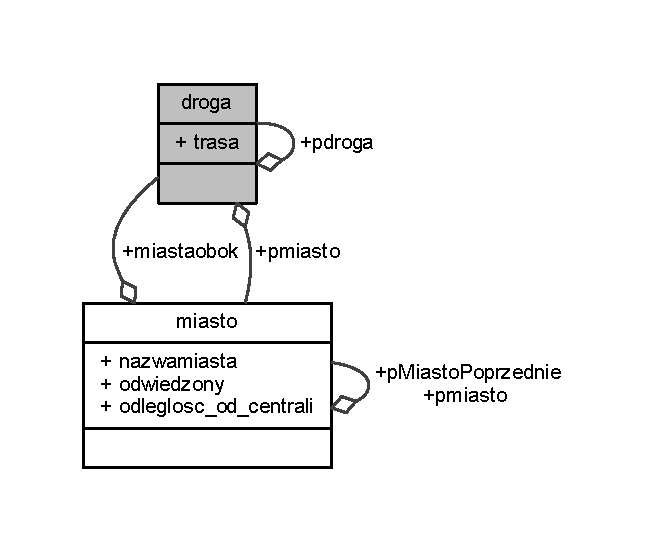
\includegraphics[width=310pt]{structdroga__coll__graph}
\end{center}
\end{figure}
\subsection*{Public Attributes}
\begin{DoxyCompactItemize}
\item 
int \mbox{\hyperlink{structdroga_a4788083344d3da2783792f80b35ab524}{trasa}}
\item 
\mbox{\hyperlink{structdroga}{droga}} $\ast$ \mbox{\hyperlink{structdroga_a7ed57ce3de3b4184ba7f7c805964626f}{pdroga}}
\item 
\mbox{\hyperlink{structmiasto}{miasto}} $\ast$ \mbox{\hyperlink{structdroga_a9c782b9f5281ee0f4cb4581a364b4471}{pmiasto}}
\end{DoxyCompactItemize}


\subsection{Detailed Description}
Struktura droga 
\begin{DoxyParams}{Parameters}
{\em trasa} & odleglosc miedzy miastami \\
\hline
{\em pdroga} & wskaznik na nastepna droge \\
\hline
{\em pmiasto} & wskaznik na odpowiednie miasto \\
\hline
\end{DoxyParams}


\subsection{Member Data Documentation}
\mbox{\Hypertarget{structdroga_a7ed57ce3de3b4184ba7f7c805964626f}\label{structdroga_a7ed57ce3de3b4184ba7f7c805964626f}} 
\index{droga@{droga}!pdroga@{pdroga}}
\index{pdroga@{pdroga}!droga@{droga}}
\subsubsection{\texorpdfstring{pdroga}{pdroga}}
{\footnotesize\ttfamily \mbox{\hyperlink{structdroga}{droga}}$\ast$ droga\+::pdroga}

\mbox{\Hypertarget{structdroga_a9c782b9f5281ee0f4cb4581a364b4471}\label{structdroga_a9c782b9f5281ee0f4cb4581a364b4471}} 
\index{droga@{droga}!pmiasto@{pmiasto}}
\index{pmiasto@{pmiasto}!droga@{droga}}
\subsubsection{\texorpdfstring{pmiasto}{pmiasto}}
{\footnotesize\ttfamily \mbox{\hyperlink{structmiasto}{miasto}}$\ast$ droga\+::pmiasto}

\mbox{\Hypertarget{structdroga_a4788083344d3da2783792f80b35ab524}\label{structdroga_a4788083344d3da2783792f80b35ab524}} 
\index{droga@{droga}!trasa@{trasa}}
\index{trasa@{trasa}!droga@{droga}}
\subsubsection{\texorpdfstring{trasa}{trasa}}
{\footnotesize\ttfamily int droga\+::trasa}



The documentation for this struct was generated from the following file\+:\begin{DoxyCompactItemize}
\item 
\mbox{\hyperlink{struktury_8h}{struktury.\+h}}\end{DoxyCompactItemize}

\hypertarget{structmiasto}{}\section{miasto Struct Reference}
\label{structmiasto}\index{miasto@{miasto}}


{\ttfamily \#include $<$struktury.\+h$>$}



Collaboration diagram for miasto\+:
% FIG 0
\subsection*{Public Attributes}
\begin{DoxyCompactItemize}
\item 
std\+::string \mbox{\hyperlink{structmiasto_a75a023beb08b889860c2068ffd47318e}{nazwamiasta}}
\item 
\mbox{\hyperlink{structmiasto}{miasto}} $\ast$ \mbox{\hyperlink{structmiasto_a9cd7b8d4e3e00ba833d3149b76a918f9}{pmiasto}}
\item 
\mbox{\hyperlink{structdroga}{droga}} $\ast$ \mbox{\hyperlink{structmiasto_af69437beea5c134e233947df273a48a4}{miastaobok}}
\item 
bool \mbox{\hyperlink{structmiasto_a7a2028174edb36e184c06d084d02ef27}{odwiedzony}}
\item 
int \mbox{\hyperlink{structmiasto_a0c3b5abe9b7ab0df2ceb80f9bd3faec3}{odleglosc\+\_\+od\+\_\+centrali}}
\item 
\mbox{\hyperlink{structmiasto}{miasto}} $\ast$ \mbox{\hyperlink{structmiasto_a8238eaa6785b35e180170ae00996e515}{p\+Miasto\+Poprzednie}}
\end{DoxyCompactItemize}


\subsection{Member Data Documentation}
\mbox{\Hypertarget{structmiasto_af69437beea5c134e233947df273a48a4}\label{structmiasto_af69437beea5c134e233947df273a48a4}} 
\index{miasto@{miasto}!miastaobok@{miastaobok}}
\index{miastaobok@{miastaobok}!miasto@{miasto}}
\subsubsection{\texorpdfstring{miastaobok}{miastaobok}}
{\footnotesize\ttfamily \mbox{\hyperlink{structdroga}{droga}}$\ast$ miasto\+::miastaobok}

\mbox{\Hypertarget{structmiasto_a75a023beb08b889860c2068ffd47318e}\label{structmiasto_a75a023beb08b889860c2068ffd47318e}} 
\index{miasto@{miasto}!nazwamiasta@{nazwamiasta}}
\index{nazwamiasta@{nazwamiasta}!miasto@{miasto}}
\subsubsection{\texorpdfstring{nazwamiasta}{nazwamiasta}}
{\footnotesize\ttfamily std\+::string miasto\+::nazwamiasta}

\mbox{\Hypertarget{structmiasto_a0c3b5abe9b7ab0df2ceb80f9bd3faec3}\label{structmiasto_a0c3b5abe9b7ab0df2ceb80f9bd3faec3}} 
\index{miasto@{miasto}!odleglosc\+\_\+od\+\_\+centrali@{odleglosc\+\_\+od\+\_\+centrali}}
\index{odleglosc\+\_\+od\+\_\+centrali@{odleglosc\+\_\+od\+\_\+centrali}!miasto@{miasto}}
\subsubsection{\texorpdfstring{odleglosc\+\_\+od\+\_\+centrali}{odleglosc\_od\_centrali}}
{\footnotesize\ttfamily int miasto\+::odleglosc\+\_\+od\+\_\+centrali}

\mbox{\Hypertarget{structmiasto_a7a2028174edb36e184c06d084d02ef27}\label{structmiasto_a7a2028174edb36e184c06d084d02ef27}} 
\index{miasto@{miasto}!odwiedzony@{odwiedzony}}
\index{odwiedzony@{odwiedzony}!miasto@{miasto}}
\subsubsection{\texorpdfstring{odwiedzony}{odwiedzony}}
{\footnotesize\ttfamily bool miasto\+::odwiedzony}

\mbox{\Hypertarget{structmiasto_a9cd7b8d4e3e00ba833d3149b76a918f9}\label{structmiasto_a9cd7b8d4e3e00ba833d3149b76a918f9}} 
\index{miasto@{miasto}!pmiasto@{pmiasto}}
\index{pmiasto@{pmiasto}!miasto@{miasto}}
\subsubsection{\texorpdfstring{pmiasto}{pmiasto}}
{\footnotesize\ttfamily \mbox{\hyperlink{structmiasto}{miasto}}$\ast$ miasto\+::pmiasto}

\mbox{\Hypertarget{structmiasto_a8238eaa6785b35e180170ae00996e515}\label{structmiasto_a8238eaa6785b35e180170ae00996e515}} 
\index{miasto@{miasto}!p\+Miasto\+Poprzednie@{p\+Miasto\+Poprzednie}}
\index{p\+Miasto\+Poprzednie@{p\+Miasto\+Poprzednie}!miasto@{miasto}}
\subsubsection{\texorpdfstring{p\+Miasto\+Poprzednie}{pMiastoPoprzednie}}
{\footnotesize\ttfamily \mbox{\hyperlink{structmiasto}{miasto}}$\ast$ miasto\+::p\+Miasto\+Poprzednie}



The documentation for this struct was generated from the following file\+:\begin{DoxyCompactItemize}
\item 
\mbox{\hyperlink{struktury_8h}{struktury.\+h}}\end{DoxyCompactItemize}

\chapter{File Documentation}
\hypertarget{_console_application1_8cpp}{}\section{Console\+Application1.\+cpp File Reference}
\label{_console_application1_8cpp}\index{Console\+Application1.\+cpp@{Console\+Application1.\+cpp}}
{\ttfamily \#include $<$iostream$>$}\newline
{\ttfamily \#include $<$fstream$>$}\newline
{\ttfamily \#include $<$string$>$}\newline
{\ttfamily \#include $<$sstream$>$}\newline
{\ttfamily \#include $<$iomanip$>$}\newline
{\ttfamily \#include $<$limits$>$}\newline
{\ttfamily \#include $<$limits.\+h$>$}\newline
{\ttfamily \#include \char`\"{}string.\+h\char`\"{}}\newline
{\ttfamily \#include \char`\"{}pch.\+h\char`\"{}}\newline
{\ttfamily \#include \char`\"{}struktury.\+h\char`\"{}}\newline
{\ttfamily \#include \char`\"{}funkcje.\+h\char`\"{}}\newline
Include dependency graph for Console\+Application1.\+cpp\+:
% FIG 0
\subsection*{Macros}
\begin{DoxyCompactItemize}
\item 
\#define \mbox{\hyperlink{_console_application1_8cpp_a1614f028c1fef258edfb81fb963609cb}{debug}}(x)~std\+::cerr $<$$<$ \char`\"{}(\char`\"{} $<$$<$ \+\_\+\+\_\+\+L\+I\+N\+E\+\_\+\+\_\+ $<$$<$ \char`\"{}) \char`\"{} $<$$<$ \#x $<$$<$ \char`\"{} == \char`\"{} $<$$<$ (x) $<$$<$ std\+::endl;
\end{DoxyCompactItemize}
\subsection*{Functions}
\begin{DoxyCompactItemize}
\item 
int \mbox{\hyperlink{_console_application1_8cpp_ab70e0563e49ae5efa9e43280907f91d7}{main}} (int ile, char $\ast$$\ast$params)
\end{DoxyCompactItemize}


\subsection{Macro Definition Documentation}
\mbox{\Hypertarget{_console_application1_8cpp_a1614f028c1fef258edfb81fb963609cb}\label{_console_application1_8cpp_a1614f028c1fef258edfb81fb963609cb}} 
\index{Console\+Application1.\+cpp@{Console\+Application1.\+cpp}!debug@{debug}}
\index{debug@{debug}!Console\+Application1.\+cpp@{Console\+Application1.\+cpp}}
\subsubsection{\texorpdfstring{debug}{debug}}
{\footnotesize\ttfamily \#define debug(\begin{DoxyParamCaption}\item[{}]{x }\end{DoxyParamCaption})~std\+::cerr $<$$<$ \char`\"{}(\char`\"{} $<$$<$ \+\_\+\+\_\+\+L\+I\+N\+E\+\_\+\+\_\+ $<$$<$ \char`\"{}) \char`\"{} $<$$<$ \#x $<$$<$ \char`\"{} == \char`\"{} $<$$<$ (x) $<$$<$ std\+::endl;}



\subsection{Function Documentation}
\mbox{\Hypertarget{_console_application1_8cpp_ab70e0563e49ae5efa9e43280907f91d7}\label{_console_application1_8cpp_ab70e0563e49ae5efa9e43280907f91d7}} 
\index{Console\+Application1.\+cpp@{Console\+Application1.\+cpp}!main@{main}}
\index{main@{main}!Console\+Application1.\+cpp@{Console\+Application1.\+cpp}}
\subsubsection{\texorpdfstring{main()}{main()}}
{\footnotesize\ttfamily int main (\begin{DoxyParamCaption}\item[{int}]{ile,  }\item[{char $\ast$$\ast$}]{params }\end{DoxyParamCaption})}

Here is the call graph for this function\+:
% FIG 1

\hypertarget{funkcje_8cpp}{}\section{Dokumentacja pliku funkcje.\+cpp}
\label{funkcje_8cpp}\index{funkcje.\+cpp@{funkcje.\+cpp}}
{\ttfamily \#include $<$iostream$>$}\newline
{\ttfamily \#include $<$fstream$>$}\newline
{\ttfamily \#include $<$string$>$}\newline
{\ttfamily \#include $<$sstream$>$}\newline
{\ttfamily \#include $<$limits$>$}\newline
{\ttfamily \#include $<$iomanip$>$}\newline
{\ttfamily \#include $<$ios$>$}\newline
{\ttfamily \#include $<$limits.\+h$>$}\newline
{\ttfamily \#include \char`\"{}pch.\+h\char`\"{}}\newline
{\ttfamily \#include \char`\"{}struktury.\+h\char`\"{}}\newline
{\ttfamily \#include \char`\"{}funkcje.\+h\char`\"{}}\newline
Wykres zależności załączania dla funkcje.\+cpp\+:\nopagebreak
\begin{figure}[H]
\begin{center}
\leavevmode
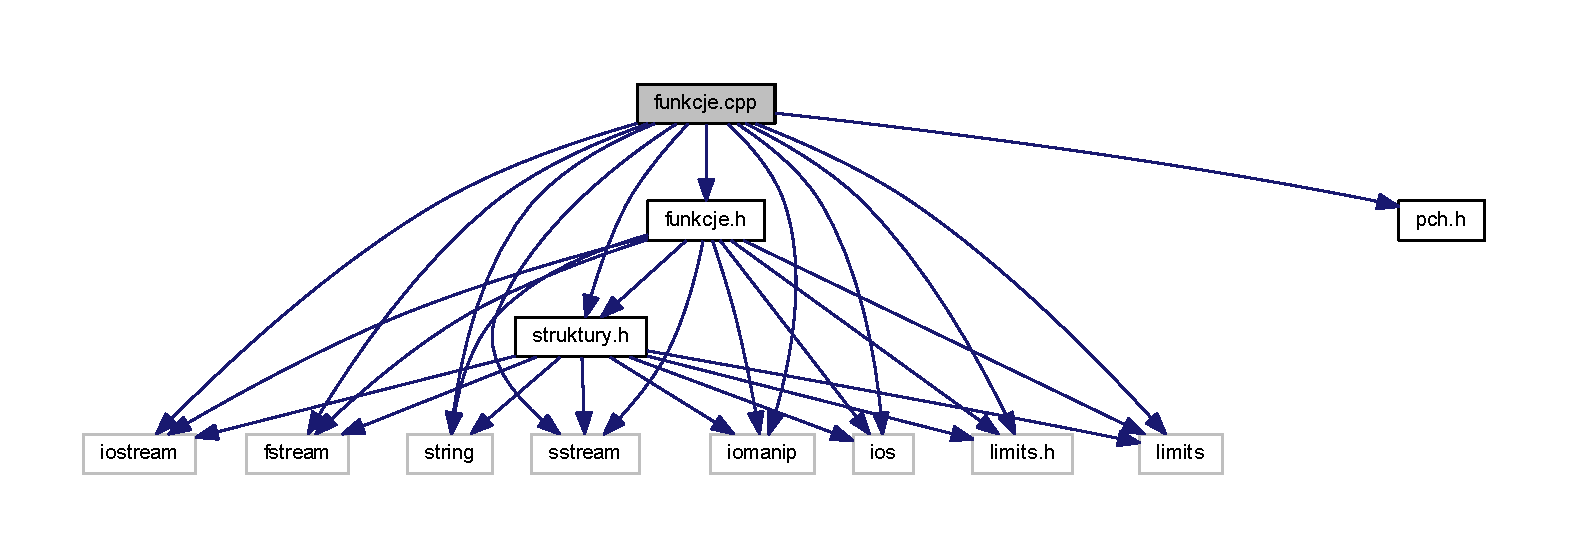
\includegraphics[width=350pt]{funkcje_8cpp__incl}
\end{center}
\end{figure}
\subsection*{Funkcje}
\begin{DoxyCompactItemize}
\item 
\mbox{\hyperlink{structmiasto}{miasto}} $\ast$ \mbox{\hyperlink{funkcje_8cpp_a65b12e45e5c2505a3f85dd606516212c}{stworz\+\_\+miasto}} (\mbox{\hyperlink{structmiasto}{miasto}} $\ast$\&p\+Head\+\_\+miasto, const std\+::string \&nowanazwa)
\item 
void \mbox{\hyperlink{funkcje_8cpp_a5861dbcdab8888ba47cb308b8f47a05a}{stworz\+\_\+droga}} (int kilometry, \mbox{\hyperlink{structmiasto}{miasto}} $\ast$\&nowe\+\_\+miasto1, \mbox{\hyperlink{structmiasto}{miasto}} $\ast$\&nowe\+\_\+miasto2)
\item 
void \mbox{\hyperlink{funkcje_8cpp_a972eb4d39e18832696cfc49a88688084}{wypisz\+\_\+droga}} (\mbox{\hyperlink{structdroga}{droga}} $\ast$p\+Head\+\_\+droga)
\item 
void \mbox{\hyperlink{funkcje_8cpp_a6aab3a8dc98794a386d900fd95c134bc}{wypisz\+\_\+miasto}} (\mbox{\hyperlink{structmiasto}{miasto}} $\ast$p\+Head)
\item 
bool \mbox{\hyperlink{funkcje_8cpp_a3ec9a37438ebb5c2e5e1b7a53b5a1198}{Dijkstra}} (const std\+::string \&startowy, \mbox{\hyperlink{structmiasto}{miasto}} $\ast$p\+Head)
\item 
void \mbox{\hyperlink{funkcje_8cpp_ae23180fadb7ac55d4d66d10ff579f16d}{wypisz\+\_\+miasta}} (\mbox{\hyperlink{structmiasto}{miasto}} $\ast$p\+Head, std\+::ostream \&wyjscie)
\item 
void \mbox{\hyperlink{funkcje_8cpp_af31b7e1c31ad3b478c612cb5a350439d}{wypisz\+\_\+wynik}} (\mbox{\hyperlink{structmiasto}{miasto}} $\ast$p\+Head, const std\+::string \&wyjscie)
\item 
bool \mbox{\hyperlink{funkcje_8cpp_a40fe3dceb03c4c0dd8aab0292c5e6ffd}{sprawdz\+\_\+argumenty}} (int ile, char $\ast$$\ast$params, std\+::string \&wejscie, std\+::string \&wyjscie, std\+::string \&start)
\item 
void \mbox{\hyperlink{funkcje_8cpp_ade295971762b742b2b2127c41c23bb11}{wczytajz\+Pliku}} (const std\+::string \&wejscie, \mbox{\hyperlink{structmiasto}{miasto}} $\ast$\&p\+Glowa)
\item 
void \mbox{\hyperlink{funkcje_8cpp_ac3ddb9423da2f8370508b4e7eeeb75f4}{usun\+\_\+drogi}} (\mbox{\hyperlink{structmiasto}{miasto}} $\ast$pmiasto)
\item 
void \mbox{\hyperlink{funkcje_8cpp_aa23ae00d9a969716225cac3bcecc6d66}{usun\+\_\+miasta}} (\mbox{\hyperlink{structmiasto}{miasto}} $\ast$\&p\+Head)
\item 
void \mbox{\hyperlink{funkcje_8cpp_a1cce16b03fb2b1138609a546417fc7dd}{usun}} (\mbox{\hyperlink{structmiasto}{miasto}} $\ast$glowa\+\_\+miasta)
\item 
void \mbox{\hyperlink{funkcje_8cpp_a6afafef7be0d9599c9e551cd4c9885bc}{help}} (int ile, char $\ast$$\ast$params)
\end{DoxyCompactItemize}


\subsection{Dokumentacja funkcji}
\mbox{\Hypertarget{funkcje_8cpp_a3ec9a37438ebb5c2e5e1b7a53b5a1198}\label{funkcje_8cpp_a3ec9a37438ebb5c2e5e1b7a53b5a1198}} 
\index{funkcje.\+cpp@{funkcje.\+cpp}!Dijkstra@{Dijkstra}}
\index{Dijkstra@{Dijkstra}!funkcje.\+cpp@{funkcje.\+cpp}}
\subsubsection{\texorpdfstring{Dijkstra()}{Dijkstra()}}
{\footnotesize\ttfamily bool Dijkstra (\begin{DoxyParamCaption}\item[{const std\+::string \&}]{startowy,  }\item[{\mbox{\hyperlink{structmiasto}{miasto}} $\ast$}]{p\+Head }\end{DoxyParamCaption})}

Funkcja, wykorzystuj�ca algorytm Dijkstry do znalezienia najkrotszych drog z miasta startowego do pozostalych miast ~\newline

\begin{DoxyParams}{Parametry}
{\em startowy} & miasto, od ktorego beda rozpoczynac sie wszystkie trasy \\
\hline
{\em p\+Head} & wskaznik na pierwszy element listy \\
\hline
\end{DoxyParams}
\begin{DoxyReturn}{Zwraca}
Funkcja zwraca true, gdy miasto startowe bylo w liscie i false, gdy nie bylo w liscie 
\end{DoxyReturn}
Oto graf wywoływań tej funkcji\+:\nopagebreak
\begin{figure}[H]
\begin{center}
\leavevmode
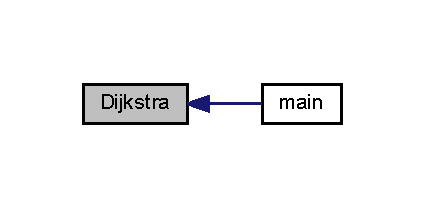
\includegraphics[width=204pt]{funkcje_8cpp_a3ec9a37438ebb5c2e5e1b7a53b5a1198_icgraph}
\end{center}
\end{figure}
\mbox{\Hypertarget{funkcje_8cpp_a6afafef7be0d9599c9e551cd4c9885bc}\label{funkcje_8cpp_a6afafef7be0d9599c9e551cd4c9885bc}} 
\index{funkcje.\+cpp@{funkcje.\+cpp}!help@{help}}
\index{help@{help}!funkcje.\+cpp@{funkcje.\+cpp}}
\subsubsection{\texorpdfstring{help()}{help()}}
{\footnotesize\ttfamily void help (\begin{DoxyParamCaption}\item[{int}]{ile,  }\item[{char $\ast$$\ast$}]{params }\end{DoxyParamCaption})}

Funkcja wyswietla pomoc 
\begin{DoxyParams}{Parametry}
{\em ile} & ilosc argumentow \\
\hline
{\em params} & tablica argumentow \\
\hline
\end{DoxyParams}
\begin{DoxyReturn}{Zwraca}
Funkcja nie zwraca niczego. 
\end{DoxyReturn}
Oto graf wywoływań tej funkcji\+:\nopagebreak
\begin{figure}[H]
\begin{center}
\leavevmode
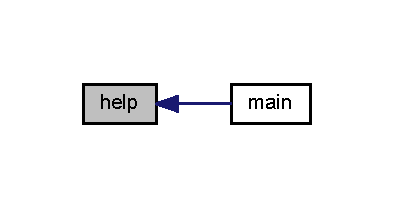
\includegraphics[width=189pt]{funkcje_8cpp_a6afafef7be0d9599c9e551cd4c9885bc_icgraph}
\end{center}
\end{figure}
\mbox{\Hypertarget{funkcje_8cpp_a40fe3dceb03c4c0dd8aab0292c5e6ffd}\label{funkcje_8cpp_a40fe3dceb03c4c0dd8aab0292c5e6ffd}} 
\index{funkcje.\+cpp@{funkcje.\+cpp}!sprawdz\+\_\+argumenty@{sprawdz\+\_\+argumenty}}
\index{sprawdz\+\_\+argumenty@{sprawdz\+\_\+argumenty}!funkcje.\+cpp@{funkcje.\+cpp}}
\subsubsection{\texorpdfstring{sprawdz\+\_\+argumenty()}{sprawdz\_argumenty()}}
{\footnotesize\ttfamily bool sprawdz\+\_\+argumenty (\begin{DoxyParamCaption}\item[{int}]{ile,  }\item[{char $\ast$$\ast$}]{params,  }\item[{std\+::string \&}]{wejscie,  }\item[{std\+::string \&}]{wyjscie,  }\item[{std\+::string \&}]{start }\end{DoxyParamCaption})}

Funkcja sprawdza argumenty wywolania programu 
\begin{DoxyParams}[1]{Parametry}
 & {\em ile} & ilosc argumentow \\
\hline
 & {\em params} & tablica argumentow \\
\hline
\mbox{\tt out}  & {\em wejscie} & plik wejsciowy \\
\hline
\mbox{\tt out}  & {\em wyjscie} & plik wyjsciowy \\
\hline
\mbox{\tt out}  & {\em start} & miasto startowe \\
\hline
\end{DoxyParams}
\begin{DoxyReturn}{Zwraca}
Funkcja zwraca true, gdy podane argumenty byly poprawne i false, gdy byly bledne 
\end{DoxyReturn}
Oto graf wywoływań tej funkcji\+:\nopagebreak
\begin{figure}[H]
\begin{center}
\leavevmode
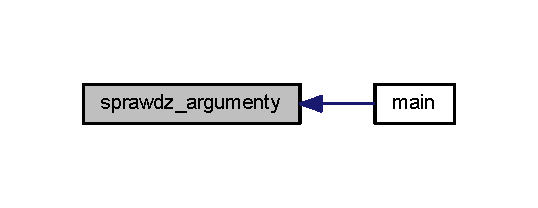
\includegraphics[width=258pt]{funkcje_8cpp_a40fe3dceb03c4c0dd8aab0292c5e6ffd_icgraph}
\end{center}
\end{figure}
\mbox{\Hypertarget{funkcje_8cpp_a5861dbcdab8888ba47cb308b8f47a05a}\label{funkcje_8cpp_a5861dbcdab8888ba47cb308b8f47a05a}} 
\index{funkcje.\+cpp@{funkcje.\+cpp}!stworz\+\_\+droga@{stworz\+\_\+droga}}
\index{stworz\+\_\+droga@{stworz\+\_\+droga}!funkcje.\+cpp@{funkcje.\+cpp}}
\subsubsection{\texorpdfstring{stworz\+\_\+droga()}{stworz\_droga()}}
{\footnotesize\ttfamily void stworz\+\_\+droga (\begin{DoxyParamCaption}\item[{int}]{kilometry,  }\item[{\mbox{\hyperlink{structmiasto}{miasto}} $\ast$\&}]{nowe\+\_\+miasto1,  }\item[{\mbox{\hyperlink{structmiasto}{miasto}} $\ast$\&}]{nowe\+\_\+miasto2 }\end{DoxyParamCaption})}

Funkcja dodaje nowe elementy do listy dr�g 
\begin{DoxyParams}{Parametry}
{\em kilometry} & odlegosc pomiedzy miastami \\
\hline
{\em nowe\+\_\+miasto1} & wskaznik na miasto poczatkowe \\
\hline
{\em nowe\+\_\+miasto2} & wskaznik na miasto docelowe \\
\hline
\end{DoxyParams}
\begin{DoxyReturn}{Zwraca}
Funkcja nie zwraca niczego. 
\end{DoxyReturn}
Oto graf wywoływań tej funkcji\+:\nopagebreak
\begin{figure}[H]
\begin{center}
\leavevmode
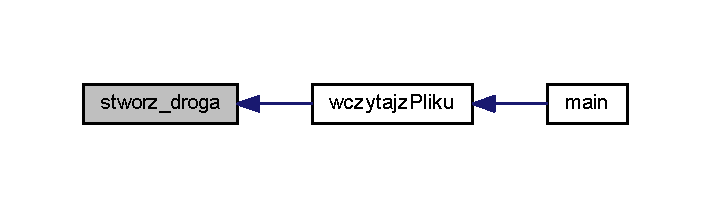
\includegraphics[width=341pt]{funkcje_8cpp_a5861dbcdab8888ba47cb308b8f47a05a_icgraph}
\end{center}
\end{figure}
\mbox{\Hypertarget{funkcje_8cpp_a65b12e45e5c2505a3f85dd606516212c}\label{funkcje_8cpp_a65b12e45e5c2505a3f85dd606516212c}} 
\index{funkcje.\+cpp@{funkcje.\+cpp}!stworz\+\_\+miasto@{stworz\+\_\+miasto}}
\index{stworz\+\_\+miasto@{stworz\+\_\+miasto}!funkcje.\+cpp@{funkcje.\+cpp}}
\subsubsection{\texorpdfstring{stworz\+\_\+miasto()}{stworz\_miasto()}}
{\footnotesize\ttfamily \mbox{\hyperlink{structmiasto}{miasto}}$\ast$ stworz\+\_\+miasto (\begin{DoxyParamCaption}\item[{\mbox{\hyperlink{structmiasto}{miasto}} $\ast$\&}]{p\+Head,  }\item[{const std\+::string \&}]{nowanazwa }\end{DoxyParamCaption})}

Funkcja dodaje nowe miasto do listy 
\begin{DoxyParams}{Parametry}
{\em p\+Head} & wskaznik na pierwszy element listy \\
\hline
{\em nowanazwa} & nazwa miasta dodawanego do listy \\
\hline
\end{DoxyParams}
\begin{DoxyReturn}{Zwraca}
Funkcja zwraca wskaznik na nowoutworzone miasto. 
\end{DoxyReturn}
Oto graf wywoływań tej funkcji\+:\nopagebreak
\begin{figure}[H]
\begin{center}
\leavevmode
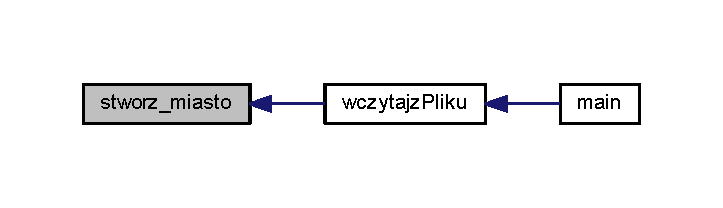
\includegraphics[width=347pt]{funkcje_8cpp_a65b12e45e5c2505a3f85dd606516212c_icgraph}
\end{center}
\end{figure}
\mbox{\Hypertarget{funkcje_8cpp_a1cce16b03fb2b1138609a546417fc7dd}\label{funkcje_8cpp_a1cce16b03fb2b1138609a546417fc7dd}} 
\index{funkcje.\+cpp@{funkcje.\+cpp}!usun@{usun}}
\index{usun@{usun}!funkcje.\+cpp@{funkcje.\+cpp}}
\subsubsection{\texorpdfstring{usun()}{usun()}}
{\footnotesize\ttfamily void usun (\begin{DoxyParamCaption}\item[{\mbox{\hyperlink{structmiasto}{miasto}} $\ast$}]{glowa\+\_\+miasta }\end{DoxyParamCaption})}

Funkcja usuwa liste miast i drog 
\begin{DoxyParams}{Parametry}
{\em glowa\+\_\+miasta} & wskaznik na pierwszy element listy miast \\
\hline
\end{DoxyParams}
\begin{DoxyReturn}{Zwraca}
Funkcja nie zwraca niczego. 
\end{DoxyReturn}
Oto graf wywołań dla tej funkcji\+:\nopagebreak
\begin{figure}[H]
\begin{center}
\leavevmode
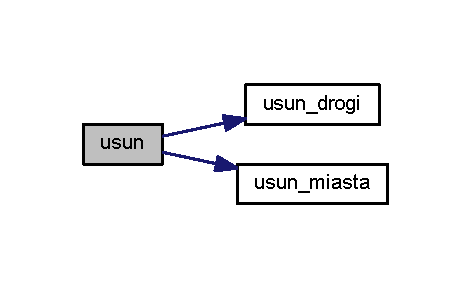
\includegraphics[width=226pt]{funkcje_8cpp_a1cce16b03fb2b1138609a546417fc7dd_cgraph}
\end{center}
\end{figure}
Oto graf wywoływań tej funkcji\+:\nopagebreak
\begin{figure}[H]
\begin{center}
\leavevmode
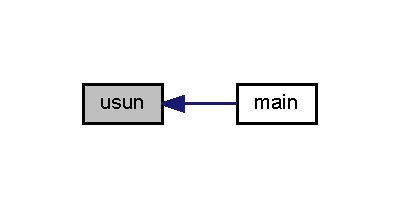
\includegraphics[width=192pt]{funkcje_8cpp_a1cce16b03fb2b1138609a546417fc7dd_icgraph}
\end{center}
\end{figure}
\mbox{\Hypertarget{funkcje_8cpp_ac3ddb9423da2f8370508b4e7eeeb75f4}\label{funkcje_8cpp_ac3ddb9423da2f8370508b4e7eeeb75f4}} 
\index{funkcje.\+cpp@{funkcje.\+cpp}!usun\+\_\+drogi@{usun\+\_\+drogi}}
\index{usun\+\_\+drogi@{usun\+\_\+drogi}!funkcje.\+cpp@{funkcje.\+cpp}}
\subsubsection{\texorpdfstring{usun\+\_\+drogi()}{usun\_drogi()}}
{\footnotesize\ttfamily void usun\+\_\+drogi (\begin{DoxyParamCaption}\item[{\mbox{\hyperlink{structmiasto}{miasto}} $\ast$}]{pmiasto }\end{DoxyParamCaption})}

Funkcja usuwa listy drog wszystkich miast 
\begin{DoxyParams}{Parametry}
{\em pmiasto} & wskaznik na kolejne miasto \\
\hline
\end{DoxyParams}
\begin{DoxyReturn}{Zwraca}
Funkcja nie zwraca niczego. 
\end{DoxyReturn}
Oto graf wywoływań tej funkcji\+:\nopagebreak
\begin{figure}[H]
\begin{center}
\leavevmode
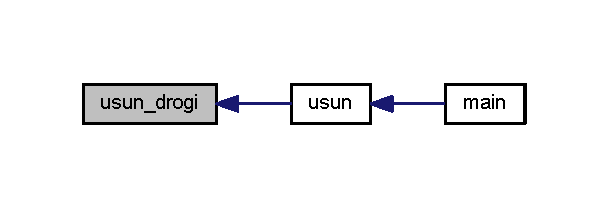
\includegraphics[width=292pt]{funkcje_8cpp_ac3ddb9423da2f8370508b4e7eeeb75f4_icgraph}
\end{center}
\end{figure}
\mbox{\Hypertarget{funkcje_8cpp_aa23ae00d9a969716225cac3bcecc6d66}\label{funkcje_8cpp_aa23ae00d9a969716225cac3bcecc6d66}} 
\index{funkcje.\+cpp@{funkcje.\+cpp}!usun\+\_\+miasta@{usun\+\_\+miasta}}
\index{usun\+\_\+miasta@{usun\+\_\+miasta}!funkcje.\+cpp@{funkcje.\+cpp}}
\subsubsection{\texorpdfstring{usun\+\_\+miasta()}{usun\_miasta()}}
{\footnotesize\ttfamily void usun\+\_\+miasta (\begin{DoxyParamCaption}\item[{\mbox{\hyperlink{structmiasto}{miasto}} $\ast$\&}]{p\+Head }\end{DoxyParamCaption})}

Funkcja usuwa liste miast 
\begin{DoxyParams}[1]{Parametry}
\mbox{\tt in,out}  & {\em p\+Head} & wskaznik na pierwszy element listy \\
\hline
\end{DoxyParams}
\begin{DoxyReturn}{Zwraca}
Funkcja nie zwraca niczego. 
\end{DoxyReturn}
Oto graf wywoływań tej funkcji\+:\nopagebreak
\begin{figure}[H]
\begin{center}
\leavevmode
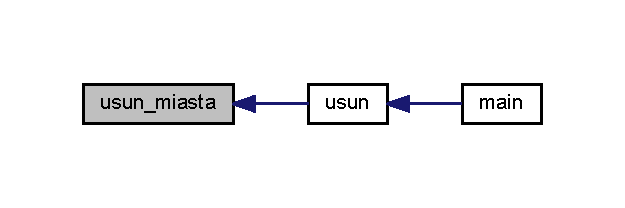
\includegraphics[width=300pt]{funkcje_8cpp_aa23ae00d9a969716225cac3bcecc6d66_icgraph}
\end{center}
\end{figure}
\mbox{\Hypertarget{funkcje_8cpp_ade295971762b742b2b2127c41c23bb11}\label{funkcje_8cpp_ade295971762b742b2b2127c41c23bb11}} 
\index{funkcje.\+cpp@{funkcje.\+cpp}!wczytajz\+Pliku@{wczytajz\+Pliku}}
\index{wczytajz\+Pliku@{wczytajz\+Pliku}!funkcje.\+cpp@{funkcje.\+cpp}}
\subsubsection{\texorpdfstring{wczytajz\+Pliku()}{wczytajzPliku()}}
{\footnotesize\ttfamily void wczytajz\+Pliku (\begin{DoxyParamCaption}\item[{const std\+::string \&}]{wejscie,  }\item[{\mbox{\hyperlink{structmiasto}{miasto}} $\ast$\&}]{p\+Glowa }\end{DoxyParamCaption})}

Funkcja wczytuje dane (miasta oraz odleglosci) z pliku 
\begin{DoxyParams}[1]{Parametry}
 & {\em wejscie} & nazwa pliku wejsciowego \\
\hline
\mbox{\tt in,out}  & {\em p\+Glowa} & wskaznik na pierwszy element listy \\
\hline
\end{DoxyParams}
Oto graf wywołań dla tej funkcji\+:\nopagebreak
\begin{figure}[H]
\begin{center}
\leavevmode
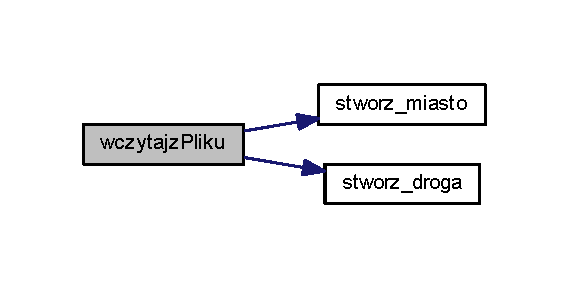
\includegraphics[width=273pt]{funkcje_8cpp_ade295971762b742b2b2127c41c23bb11_cgraph}
\end{center}
\end{figure}
Oto graf wywoływań tej funkcji\+:\nopagebreak
\begin{figure}[H]
\begin{center}
\leavevmode
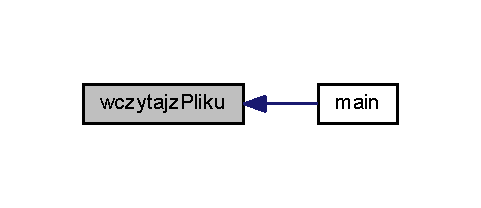
\includegraphics[width=231pt]{funkcje_8cpp_ade295971762b742b2b2127c41c23bb11_icgraph}
\end{center}
\end{figure}
\mbox{\Hypertarget{funkcje_8cpp_a972eb4d39e18832696cfc49a88688084}\label{funkcje_8cpp_a972eb4d39e18832696cfc49a88688084}} 
\index{funkcje.\+cpp@{funkcje.\+cpp}!wypisz\+\_\+droga@{wypisz\+\_\+droga}}
\index{wypisz\+\_\+droga@{wypisz\+\_\+droga}!funkcje.\+cpp@{funkcje.\+cpp}}
\subsubsection{\texorpdfstring{wypisz\+\_\+droga()}{wypisz\_droga()}}
{\footnotesize\ttfamily void wypisz\+\_\+droga (\begin{DoxyParamCaption}\item[{\mbox{\hyperlink{structdroga}{droga}} $\ast$}]{p\+Head\+\_\+droga }\end{DoxyParamCaption})}

Funkcja wypisuje liste drog 
\begin{DoxyParams}{Parametry}
{\em p\+Head\+\_\+droga} & wskaznik na pierwszy element listy \\
\hline
\end{DoxyParams}
\begin{DoxyReturn}{Zwraca}
Funkcja nie zwraca niczego. 
\end{DoxyReturn}
Oto graf wywoływań tej funkcji\+:\nopagebreak
\begin{figure}[H]
\begin{center}
\leavevmode
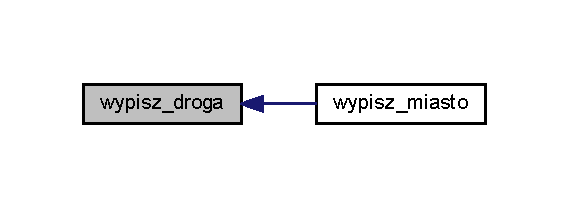
\includegraphics[width=273pt]{funkcje_8cpp_a972eb4d39e18832696cfc49a88688084_icgraph}
\end{center}
\end{figure}
\mbox{\Hypertarget{funkcje_8cpp_ae23180fadb7ac55d4d66d10ff579f16d}\label{funkcje_8cpp_ae23180fadb7ac55d4d66d10ff579f16d}} 
\index{funkcje.\+cpp@{funkcje.\+cpp}!wypisz\+\_\+miasta@{wypisz\+\_\+miasta}}
\index{wypisz\+\_\+miasta@{wypisz\+\_\+miasta}!funkcje.\+cpp@{funkcje.\+cpp}}
\subsubsection{\texorpdfstring{wypisz\+\_\+miasta()}{wypisz\_miasta()}}
{\footnotesize\ttfamily void wypisz\+\_\+miasta (\begin{DoxyParamCaption}\item[{\mbox{\hyperlink{structmiasto}{miasto}} $\ast$}]{p\+Head,  }\item[{std\+::ostream \&}]{wyjscie }\end{DoxyParamCaption})}

Funkcja wypisuje trase do wskazanego miasta ~\newline

\begin{DoxyParams}{Parametry}
{\em p\+Head} & wskaznik na pierwszy element listy \\
\hline
{\em wyjscie} & nazwa pliku wyjsciowego \\
\hline
\end{DoxyParams}
\begin{DoxyReturn}{Zwraca}
Funkcja nie zwraca niczego. 
\end{DoxyReturn}
Oto graf wywołań dla tej funkcji\+:\nopagebreak
\begin{figure}[H]
\begin{center}
\leavevmode
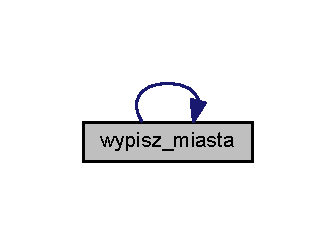
\includegraphics[width=161pt]{funkcje_8cpp_ae23180fadb7ac55d4d66d10ff579f16d_cgraph}
\end{center}
\end{figure}
Oto graf wywoływań tej funkcji\+:\nopagebreak
\begin{figure}[H]
\begin{center}
\leavevmode
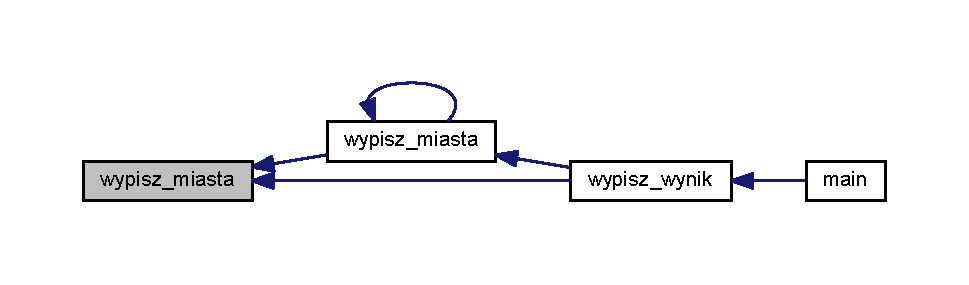
\includegraphics[width=350pt]{funkcje_8cpp_ae23180fadb7ac55d4d66d10ff579f16d_icgraph}
\end{center}
\end{figure}
\mbox{\Hypertarget{funkcje_8cpp_a6aab3a8dc98794a386d900fd95c134bc}\label{funkcje_8cpp_a6aab3a8dc98794a386d900fd95c134bc}} 
\index{funkcje.\+cpp@{funkcje.\+cpp}!wypisz\+\_\+miasto@{wypisz\+\_\+miasto}}
\index{wypisz\+\_\+miasto@{wypisz\+\_\+miasto}!funkcje.\+cpp@{funkcje.\+cpp}}
\subsubsection{\texorpdfstring{wypisz\+\_\+miasto()}{wypisz\_miasto()}}
{\footnotesize\ttfamily void wypisz\+\_\+miasto (\begin{DoxyParamCaption}\item[{\mbox{\hyperlink{structmiasto}{miasto}} $\ast$}]{p\+Head }\end{DoxyParamCaption})}

Funkcja wypisuje liste miast 
\begin{DoxyParams}{Parametry}
{\em p\+Head} & wskaznik na pierwszy element listy \\
\hline
\end{DoxyParams}
\begin{DoxyReturn}{Zwraca}
Funkcja nie zwraca niczego. 
\end{DoxyReturn}
Oto graf wywołań dla tej funkcji\+:\nopagebreak
\begin{figure}[H]
\begin{center}
\leavevmode
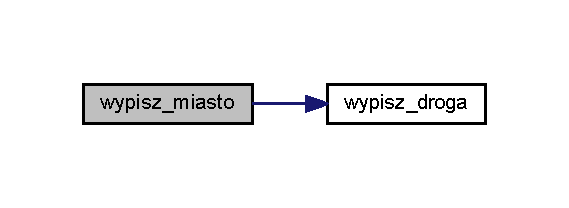
\includegraphics[width=273pt]{funkcje_8cpp_a6aab3a8dc98794a386d900fd95c134bc_cgraph}
\end{center}
\end{figure}
\mbox{\Hypertarget{funkcje_8cpp_af31b7e1c31ad3b478c612cb5a350439d}\label{funkcje_8cpp_af31b7e1c31ad3b478c612cb5a350439d}} 
\index{funkcje.\+cpp@{funkcje.\+cpp}!wypisz\+\_\+wynik@{wypisz\+\_\+wynik}}
\index{wypisz\+\_\+wynik@{wypisz\+\_\+wynik}!funkcje.\+cpp@{funkcje.\+cpp}}
\subsubsection{\texorpdfstring{wypisz\+\_\+wynik()}{wypisz\_wynik()}}
{\footnotesize\ttfamily void wypisz\+\_\+wynik (\begin{DoxyParamCaption}\item[{\mbox{\hyperlink{structmiasto}{miasto}} $\ast$}]{p\+Head,  }\item[{const std\+::string \&}]{wyjscie }\end{DoxyParamCaption})}

Funkcja zapisuje wynik (wszystkie trasy do miast wraz z odleglosciami) do pliku wyjsciowego ~\newline

\begin{DoxyParams}{Parametry}
{\em p\+Head} & wskaznik na pierwszy element listy \\
\hline
{\em wyjscie} & nazwa pliku wyjsciowego \\
\hline
\end{DoxyParams}
\begin{DoxyReturn}{Zwraca}
Funkcja nie zwraca niczego. 
\end{DoxyReturn}
Oto graf wywołań dla tej funkcji\+:\nopagebreak
\begin{figure}[H]
\begin{center}
\leavevmode
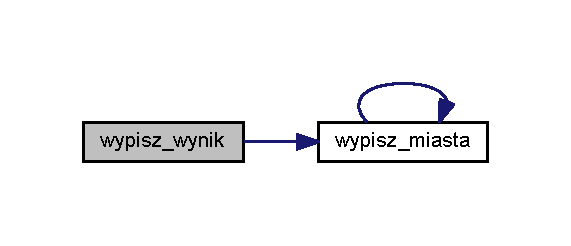
\includegraphics[width=274pt]{funkcje_8cpp_af31b7e1c31ad3b478c612cb5a350439d_cgraph}
\end{center}
\end{figure}
Oto graf wywoływań tej funkcji\+:\nopagebreak
\begin{figure}[H]
\begin{center}
\leavevmode
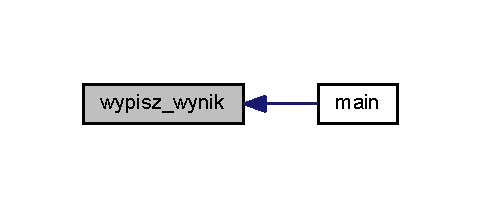
\includegraphics[width=231pt]{funkcje_8cpp_af31b7e1c31ad3b478c612cb5a350439d_icgraph}
\end{center}
\end{figure}

\hypertarget{funkcje_8h}{}\section{funkcje.\+h File Reference}
\label{funkcje_8h}\index{funkcje.\+h@{funkcje.\+h}}
{\ttfamily \#include $<$iostream$>$}\newline
{\ttfamily \#include $<$fstream$>$}\newline
{\ttfamily \#include $<$string$>$}\newline
{\ttfamily \#include $<$sstream$>$}\newline
{\ttfamily \#include $<$iomanip$>$}\newline
{\ttfamily \#include $<$limits$>$}\newline
{\ttfamily \#include $<$ios$>$}\newline
{\ttfamily \#include $<$limits.\+h$>$}\newline
{\ttfamily \#include \char`\"{}struktury.\+h\char`\"{}}\newline
Include dependency graph for funkcje.\+h\+:
% FIG 0
This graph shows which files directly or indirectly include this file\+:
% FIG 1
\subsection*{Macros}
\begin{DoxyCompactItemize}
\item 
\#define \mbox{\hyperlink{funkcje_8h_a9c6a3a9ed8523f0a4e5e8457ff99d0f8}{funkcje\+\_\+H}}
\end{DoxyCompactItemize}
\subsection*{Functions}
\begin{DoxyCompactItemize}
\item 
\mbox{\hyperlink{structmiasto}{miasto}} $\ast$ \mbox{\hyperlink{funkcje_8h_a73095f97a16eb130a65981e7fe5f05ef}{stworz\+\_\+miasto}} (\mbox{\hyperlink{structmiasto}{miasto}} $\ast$\&p\+Head, std\+::string nowanazwa)
\item 
void \mbox{\hyperlink{funkcje_8h_a7389ce903c9071cc811a37b10910a416}{stworz\+\_\+droga}} (\mbox{\hyperlink{structmiasto}{miasto}} $\ast$\&p\+Head\+\_\+miasto, int kilometry, \mbox{\hyperlink{structmiasto}{miasto}} $\ast$\&nowe\+\_\+miasto1, \mbox{\hyperlink{structmiasto}{miasto}} $\ast$\&nowe\+\_\+miasto2)
\item 
void \mbox{\hyperlink{funkcje_8h_a6aab3a8dc98794a386d900fd95c134bc}{wypisz\+\_\+miasto}} (\mbox{\hyperlink{structmiasto}{miasto}} $\ast$p\+Head)
\item 
void \mbox{\hyperlink{funkcje_8h_a972eb4d39e18832696cfc49a88688084}{wypisz\+\_\+droga}} (\mbox{\hyperlink{structdroga}{droga}} $\ast$p\+Head\+\_\+droga)
\item 
void \mbox{\hyperlink{funkcje_8h_a5fc34203e5ac8fbcf09a97be9324baae}{algorytm}} (std\+::string startowy, \mbox{\hyperlink{structmiasto}{miasto}} $\ast$\&p\+Head)
\item 
void \mbox{\hyperlink{funkcje_8h_a32b280db3bcb057f8e817d25e38a27b1}{wypisz\+\_\+wynik}} (\mbox{\hyperlink{structmiasto}{miasto}} $\ast$p\+Head, std\+::string wyjscie)
\item 
void \mbox{\hyperlink{funkcje_8h_ae23180fadb7ac55d4d66d10ff579f16d}{wypisz\+\_\+miasta}} (\mbox{\hyperlink{structmiasto}{miasto}} $\ast$p\+Head, std\+::ostream \&wyjscie)
\item 
bool \mbox{\hyperlink{funkcje_8h_a40fe3dceb03c4c0dd8aab0292c5e6ffd}{sprawdz\+\_\+argumenty}} (int ile, char $\ast$$\ast$params, std\+::string \&wejscie, std\+::string \&wyjscie, std\+::string \&start)
\item 
void \mbox{\hyperlink{funkcje_8h_a6975d209e2b2997bdef356d244dd3a6e}{wczytajz\+Pliku}} (std\+::string wejscie, \mbox{\hyperlink{structmiasto}{miasto}} $\ast$\&p\+Glowa)
\item 
void \mbox{\hyperlink{funkcje_8h_ac0a252aeb91478531356e348d2154d3d}{usun\+\_\+droge}} (\mbox{\hyperlink{structmiasto}{miasto}} $\ast$pmiasto)
\item 
void \mbox{\hyperlink{funkcje_8h_aa23ae00d9a969716225cac3bcecc6d66}{usun\+\_\+miasta}} (\mbox{\hyperlink{structmiasto}{miasto}} $\ast$\&p\+Head)
\item 
void \mbox{\hyperlink{funkcje_8h_a1cce16b03fb2b1138609a546417fc7dd}{usun}} (\mbox{\hyperlink{structmiasto}{miasto}} $\ast$glowa\+\_\+miasta)
\end{DoxyCompactItemize}


\subsection{Macro Definition Documentation}
\mbox{\Hypertarget{funkcje_8h_a9c6a3a9ed8523f0a4e5e8457ff99d0f8}\label{funkcje_8h_a9c6a3a9ed8523f0a4e5e8457ff99d0f8}} 
\index{funkcje.\+h@{funkcje.\+h}!funkcje\+\_\+H@{funkcje\+\_\+H}}
\index{funkcje\+\_\+H@{funkcje\+\_\+H}!funkcje.\+h@{funkcje.\+h}}
\subsubsection{\texorpdfstring{funkcje\+\_\+H}{funkcje\_H}}
{\footnotesize\ttfamily \#define funkcje\+\_\+H}



\subsection{Function Documentation}
\mbox{\Hypertarget{funkcje_8h_a5fc34203e5ac8fbcf09a97be9324baae}\label{funkcje_8h_a5fc34203e5ac8fbcf09a97be9324baae}} 
\index{funkcje.\+h@{funkcje.\+h}!algorytm@{algorytm}}
\index{algorytm@{algorytm}!funkcje.\+h@{funkcje.\+h}}
\subsubsection{\texorpdfstring{algorytm()}{algorytm()}}
{\footnotesize\ttfamily void algorytm (\begin{DoxyParamCaption}\item[{std\+::string}]{startowy,  }\item[{\mbox{\hyperlink{structmiasto}{miasto}} $\ast$\&}]{p\+Head }\end{DoxyParamCaption})}

Funkcja znajduje najkrotsza droge z miasta startowego do pozostalych miast 
\begin{DoxyParams}{Parameters}
{\em startowy} & miasto, od ktorego beda rozpoczynac sie wszystkie trasy \\
\hline
{\em p\+Head} & wskaznik na pierwszy element listy \\
\hline
\end{DoxyParams}
\begin{DoxyReturn}{Returns}
Funkcja nie zwraca niczego. 
\end{DoxyReturn}
Here is the caller graph for this function\+:
% FIG 2
\mbox{\Hypertarget{funkcje_8h_a40fe3dceb03c4c0dd8aab0292c5e6ffd}\label{funkcje_8h_a40fe3dceb03c4c0dd8aab0292c5e6ffd}} 
\index{funkcje.\+h@{funkcje.\+h}!sprawdz\+\_\+argumenty@{sprawdz\+\_\+argumenty}}
\index{sprawdz\+\_\+argumenty@{sprawdz\+\_\+argumenty}!funkcje.\+h@{funkcje.\+h}}
\subsubsection{\texorpdfstring{sprawdz\+\_\+argumenty()}{sprawdz\_argumenty()}}
{\footnotesize\ttfamily bool sprawdz\+\_\+argumenty (\begin{DoxyParamCaption}\item[{int}]{ile,  }\item[{char $\ast$$\ast$}]{params,  }\item[{std\+::string \&}]{wejscie,  }\item[{std\+::string \&}]{wyjscie,  }\item[{std\+::string \&}]{start }\end{DoxyParamCaption})}

Funkcja sprawdza argumenty wywolania programu 
\begin{DoxyParams}[1]{Parameters}
 & {\em ile} & ilosc argumentow \\
\hline
 & {\em params} & tablica argumentow \\
\hline
\mbox{\tt out}  & {\em wejscie} & plik wejsciowy \\
\hline
\mbox{\tt out}  & {\em wyjscie} & plik wyjsciowy \\
\hline
\mbox{\tt out}  & {\em start} & miasto startowe \\
\hline
\end{DoxyParams}
\begin{DoxyReturn}{Returns}
Funkcja nie zwraca niczego. 
\end{DoxyReturn}
Here is the caller graph for this function\+:
% FIG 3
\mbox{\Hypertarget{funkcje_8h_a7389ce903c9071cc811a37b10910a416}\label{funkcje_8h_a7389ce903c9071cc811a37b10910a416}} 
\index{funkcje.\+h@{funkcje.\+h}!stworz\+\_\+droga@{stworz\+\_\+droga}}
\index{stworz\+\_\+droga@{stworz\+\_\+droga}!funkcje.\+h@{funkcje.\+h}}
\subsubsection{\texorpdfstring{stworz\+\_\+droga()}{stworz\_droga()}}
{\footnotesize\ttfamily void stworz\+\_\+droga (\begin{DoxyParamCaption}\item[{\mbox{\hyperlink{structmiasto}{miasto}} $\ast$\&}]{p\+Head\+\_\+miasto,  }\item[{int}]{kilometry,  }\item[{\mbox{\hyperlink{structmiasto}{miasto}} $\ast$\&}]{nowe\+\_\+miasto1,  }\item[{\mbox{\hyperlink{structmiasto}{miasto}} $\ast$\&}]{nowe\+\_\+miasto2 }\end{DoxyParamCaption})}

Funkcja dodaje do listy miasta polaczone z 
\begin{DoxyParams}{Parameters}
{\em p\+Head\+\_\+miasto} & wskaznik na pierwszy element listy \\
\hline
{\em kilometry} & odlegosc pomiedzy miastami \\
\hline
{\em nowe\+\_\+miasto1} & wskaznik na miasto poczatkowe \\
\hline
{\em nowe\+\_\+miasto2} & wskaznik na miasto docelowe \\
\hline
\end{DoxyParams}
\begin{DoxyReturn}{Returns}
Funkcja nie zwraca niczego. 
\end{DoxyReturn}
Here is the caller graph for this function\+:
% FIG 4
\mbox{\Hypertarget{funkcje_8h_a73095f97a16eb130a65981e7fe5f05ef}\label{funkcje_8h_a73095f97a16eb130a65981e7fe5f05ef}} 
\index{funkcje.\+h@{funkcje.\+h}!stworz\+\_\+miasto@{stworz\+\_\+miasto}}
\index{stworz\+\_\+miasto@{stworz\+\_\+miasto}!funkcje.\+h@{funkcje.\+h}}
\subsubsection{\texorpdfstring{stworz\+\_\+miasto()}{stworz\_miasto()}}
{\footnotesize\ttfamily \mbox{\hyperlink{structmiasto}{miasto}}$\ast$ stworz\+\_\+miasto (\begin{DoxyParamCaption}\item[{\mbox{\hyperlink{structmiasto}{miasto}} $\ast$\&}]{p\+Head,  }\item[{std\+::string}]{nowanazwa }\end{DoxyParamCaption})}

Funkcja dodaje nowe miasto do listy 
\begin{DoxyParams}{Parameters}
{\em p\+Head} & wskaznik na pierwszy element listy \\
\hline
{\em nowanazwa} & nazwa miasta dodawanego do listy \\
\hline
\end{DoxyParams}
\begin{DoxyReturn}{Returns}
Funkcja zwraca wska�nik na nowoutworzone miasto. 
\end{DoxyReturn}
Here is the caller graph for this function\+:
% FIG 5
\mbox{\Hypertarget{funkcje_8h_a1cce16b03fb2b1138609a546417fc7dd}\label{funkcje_8h_a1cce16b03fb2b1138609a546417fc7dd}} 
\index{funkcje.\+h@{funkcje.\+h}!usun@{usun}}
\index{usun@{usun}!funkcje.\+h@{funkcje.\+h}}
\subsubsection{\texorpdfstring{usun()}{usun()}}
{\footnotesize\ttfamily void usun (\begin{DoxyParamCaption}\item[{\mbox{\hyperlink{structmiasto}{miasto}} $\ast$}]{glowa\+\_\+miasta }\end{DoxyParamCaption})}

Funkcja usuwa liste miast i drog 
\begin{DoxyParams}{Parameters}
{\em glowa\+\_\+miasta} & wskaznik na pierwszy element listy miast \\
\hline
\end{DoxyParams}
\begin{DoxyReturn}{Returns}
Funkcja nie zwraca niczego. 
\end{DoxyReturn}
Here is the call graph for this function\+:
% FIG 6
Here is the caller graph for this function\+:
% FIG 7
\mbox{\Hypertarget{funkcje_8h_ac0a252aeb91478531356e348d2154d3d}\label{funkcje_8h_ac0a252aeb91478531356e348d2154d3d}} 
\index{funkcje.\+h@{funkcje.\+h}!usun\+\_\+droge@{usun\+\_\+droge}}
\index{usun\+\_\+droge@{usun\+\_\+droge}!funkcje.\+h@{funkcje.\+h}}
\subsubsection{\texorpdfstring{usun\+\_\+droge()}{usun\_droge()}}
{\footnotesize\ttfamily void usun\+\_\+droge (\begin{DoxyParamCaption}\item[{\mbox{\hyperlink{structmiasto}{miasto}} $\ast$}]{pmiasto }\end{DoxyParamCaption})}

Funkcja usuwa liste drog 
\begin{DoxyParams}{Parameters}
{\em pmiasto} & wskaznik na kolejne miasto \\
\hline
\end{DoxyParams}
\begin{DoxyReturn}{Returns}
Funkcja nie zwraca niczego. 
\end{DoxyReturn}
Here is the caller graph for this function\+:
% FIG 8
\mbox{\Hypertarget{funkcje_8h_aa23ae00d9a969716225cac3bcecc6d66}\label{funkcje_8h_aa23ae00d9a969716225cac3bcecc6d66}} 
\index{funkcje.\+h@{funkcje.\+h}!usun\+\_\+miasta@{usun\+\_\+miasta}}
\index{usun\+\_\+miasta@{usun\+\_\+miasta}!funkcje.\+h@{funkcje.\+h}}
\subsubsection{\texorpdfstring{usun\+\_\+miasta()}{usun\_miasta()}}
{\footnotesize\ttfamily void usun\+\_\+miasta (\begin{DoxyParamCaption}\item[{\mbox{\hyperlink{structmiasto}{miasto}} $\ast$\&}]{p\+Head }\end{DoxyParamCaption})}

Funkcja usuwa liste miast 
\begin{DoxyParams}{Parameters}
{\em p\+Head} & wskaznik na pierwszy element listy \\
\hline
\end{DoxyParams}
\begin{DoxyReturn}{Returns}
Funkcja nie zwraca niczego. 
\end{DoxyReturn}
Here is the caller graph for this function\+:
% FIG 9
\mbox{\Hypertarget{funkcje_8h_a6975d209e2b2997bdef356d244dd3a6e}\label{funkcje_8h_a6975d209e2b2997bdef356d244dd3a6e}} 
\index{funkcje.\+h@{funkcje.\+h}!wczytajz\+Pliku@{wczytajz\+Pliku}}
\index{wczytajz\+Pliku@{wczytajz\+Pliku}!funkcje.\+h@{funkcje.\+h}}
\subsubsection{\texorpdfstring{wczytajz\+Pliku()}{wczytajzPliku()}}
{\footnotesize\ttfamily void wczytajz\+Pliku (\begin{DoxyParamCaption}\item[{std\+::string}]{wejscie,  }\item[{\mbox{\hyperlink{structmiasto}{miasto}} $\ast$\&}]{p\+Glowa }\end{DoxyParamCaption})}

Funkcja wczytuje dane z pliku 
\begin{DoxyParams}{Parameters}
{\em wejscie} & nazwa pliku wejsciowego \\
\hline
{\em p\+Glowa} & wskaznik na pierwszy element listy \\
\hline
\end{DoxyParams}
Here is the call graph for this function\+:
% FIG 10
Here is the caller graph for this function\+:
% FIG 11
\mbox{\Hypertarget{funkcje_8h_a972eb4d39e18832696cfc49a88688084}\label{funkcje_8h_a972eb4d39e18832696cfc49a88688084}} 
\index{funkcje.\+h@{funkcje.\+h}!wypisz\+\_\+droga@{wypisz\+\_\+droga}}
\index{wypisz\+\_\+droga@{wypisz\+\_\+droga}!funkcje.\+h@{funkcje.\+h}}
\subsubsection{\texorpdfstring{wypisz\+\_\+droga()}{wypisz\_droga()}}
{\footnotesize\ttfamily void wypisz\+\_\+droga (\begin{DoxyParamCaption}\item[{\mbox{\hyperlink{structdroga}{droga}} $\ast$}]{p\+Head\+\_\+droga }\end{DoxyParamCaption})}

Funkcja wypisuje liste drog 
\begin{DoxyParams}{Parameters}
{\em p\+Head\+\_\+droga} & wskaznik na pierwszy element listy \\
\hline
\end{DoxyParams}
\begin{DoxyReturn}{Returns}
Funkcja nie zwraca niczego. 
\end{DoxyReturn}
Here is the caller graph for this function\+:
% FIG 12
\mbox{\Hypertarget{funkcje_8h_ae23180fadb7ac55d4d66d10ff579f16d}\label{funkcje_8h_ae23180fadb7ac55d4d66d10ff579f16d}} 
\index{funkcje.\+h@{funkcje.\+h}!wypisz\+\_\+miasta@{wypisz\+\_\+miasta}}
\index{wypisz\+\_\+miasta@{wypisz\+\_\+miasta}!funkcje.\+h@{funkcje.\+h}}
\subsubsection{\texorpdfstring{wypisz\+\_\+miasta()}{wypisz\_miasta()}}
{\footnotesize\ttfamily void wypisz\+\_\+miasta (\begin{DoxyParamCaption}\item[{\mbox{\hyperlink{structmiasto}{miasto}} $\ast$}]{p\+Head,  }\item[{std\+::ostream \&}]{wyjscie }\end{DoxyParamCaption})}

Funkcja zapisuje trasy do pliku wyjsciowego ~\newline

\begin{DoxyParams}{Parameters}
{\em p\+Head} & wskaznik na pierwszy element listy \\
\hline
{\em wyjscie} & nazwa pliku wyjsciowego \\
\hline
\end{DoxyParams}
\begin{DoxyReturn}{Returns}
Funkcja nie zwraca niczego. 
\end{DoxyReturn}
Here is the call graph for this function\+:
% FIG 13
Here is the caller graph for this function\+:
% FIG 14
\mbox{\Hypertarget{funkcje_8h_a6aab3a8dc98794a386d900fd95c134bc}\label{funkcje_8h_a6aab3a8dc98794a386d900fd95c134bc}} 
\index{funkcje.\+h@{funkcje.\+h}!wypisz\+\_\+miasto@{wypisz\+\_\+miasto}}
\index{wypisz\+\_\+miasto@{wypisz\+\_\+miasto}!funkcje.\+h@{funkcje.\+h}}
\subsubsection{\texorpdfstring{wypisz\+\_\+miasto()}{wypisz\_miasto()}}
{\footnotesize\ttfamily void wypisz\+\_\+miasto (\begin{DoxyParamCaption}\item[{\mbox{\hyperlink{structmiasto}{miasto}} $\ast$}]{p\+Head }\end{DoxyParamCaption})}

Funkcja wypisuje liste miast 
\begin{DoxyParams}{Parameters}
{\em p\+Head} & wskaznik na pierwszy element listy \\
\hline
\end{DoxyParams}
\begin{DoxyReturn}{Returns}
Funkcja nie zwraca niczego. 
\end{DoxyReturn}
Here is the call graph for this function\+:
% FIG 15
\mbox{\Hypertarget{funkcje_8h_a32b280db3bcb057f8e817d25e38a27b1}\label{funkcje_8h_a32b280db3bcb057f8e817d25e38a27b1}} 
\index{funkcje.\+h@{funkcje.\+h}!wypisz\+\_\+wynik@{wypisz\+\_\+wynik}}
\index{wypisz\+\_\+wynik@{wypisz\+\_\+wynik}!funkcje.\+h@{funkcje.\+h}}
\subsubsection{\texorpdfstring{wypisz\+\_\+wynik()}{wypisz\_wynik()}}
{\footnotesize\ttfamily void wypisz\+\_\+wynik (\begin{DoxyParamCaption}\item[{\mbox{\hyperlink{structmiasto}{miasto}} $\ast$}]{p\+Head,  }\item[{std\+::string}]{wyjscie }\end{DoxyParamCaption})}

Funkcja zapisuje wynik do pliku wyjsciowego ~\newline

\begin{DoxyParams}{Parameters}
{\em p\+Head} & wskaznik na pierwszy element listy \\
\hline
{\em wyjscie} & nazwa pliku wyjsciowego \\
\hline
\end{DoxyParams}
\begin{DoxyReturn}{Returns}
Funkcja nie zwraca niczego. 
\end{DoxyReturn}
Here is the call graph for this function\+:
% FIG 16
Here is the caller graph for this function\+:
% FIG 17

\hypertarget{pch_8cpp}{}\section{pch.\+cpp File Reference}
\label{pch_8cpp}\index{pch.\+cpp@{pch.\+cpp}}
{\ttfamily \#include \char`\"{}pch.\+h\char`\"{}}\newline
Include dependency graph for pch.\+cpp\+:
\nopagebreak
\begin{figure}[H]
\begin{center}
\leavevmode
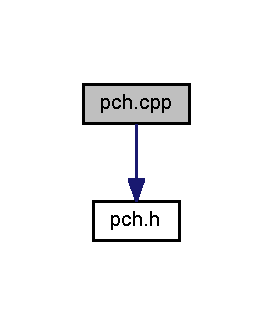
\includegraphics[width=131pt]{pch_8cpp__incl}
\end{center}
\end{figure}

\hypertarget{pch_8h}{}\section{pch.\+h File Reference}
\label{pch_8h}\index{pch.\+h@{pch.\+h}}
This graph shows which files directly or indirectly include this file\+:
% FIG 0

\hypertarget{struktury_8cpp}{}\section{struktury.\+cpp File Reference}
\label{struktury_8cpp}\index{struktury.\+cpp@{struktury.\+cpp}}
{\ttfamily \#include $<$iostream$>$}\newline
{\ttfamily \#include $<$fstream$>$}\newline
{\ttfamily \#include $<$string$>$}\newline
{\ttfamily \#include $<$sstream$>$}\newline
{\ttfamily \#include $<$iomanip$>$}\newline
{\ttfamily \#include \char`\"{}pch.\+h\char`\"{}}\newline
{\ttfamily \#include \char`\"{}struktury.\+h\char`\"{}}\newline
{\ttfamily \#include \char`\"{}funkcje.\+h\char`\"{}}\newline
Include dependency graph for struktury.\+cpp\+:
\nopagebreak
\begin{figure}[H]
\begin{center}
\leavevmode
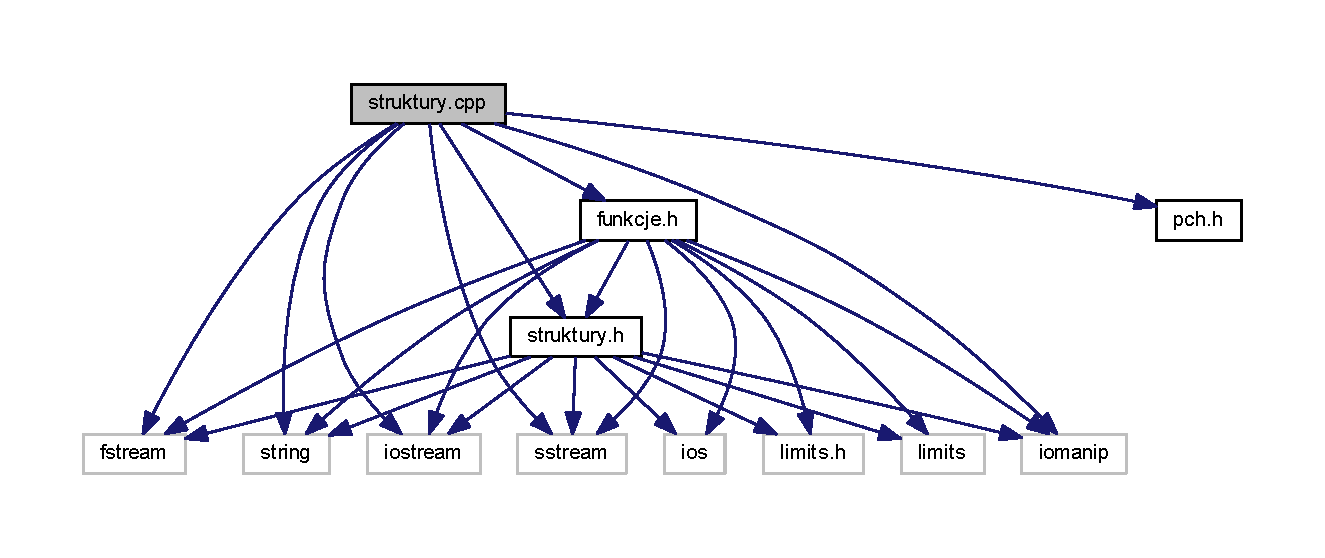
\includegraphics[width=350pt]{struktury_8cpp__incl}
\end{center}
\end{figure}

\hypertarget{struktury_8h}{}\section{struktury.\+h File Reference}
\label{struktury_8h}\index{struktury.\+h@{struktury.\+h}}
{\ttfamily \#include $<$iostream$>$}\newline
{\ttfamily \#include $<$fstream$>$}\newline
{\ttfamily \#include $<$string$>$}\newline
{\ttfamily \#include $<$sstream$>$}\newline
{\ttfamily \#include $<$iomanip$>$}\newline
{\ttfamily \#include $<$limits$>$}\newline
{\ttfamily \#include $<$ios$>$}\newline
{\ttfamily \#include $<$limits.\+h$>$}\newline
Include dependency graph for struktury.\+h\+:
% FIG 0
This graph shows which files directly or indirectly include this file\+:
% FIG 1
\subsection*{Classes}
\begin{DoxyCompactItemize}
\item 
struct \mbox{\hyperlink{structmiasto}{miasto}}
\item 
struct \mbox{\hyperlink{structdroga}{droga}}
\end{DoxyCompactItemize}
\subsection*{Macros}
\begin{DoxyCompactItemize}
\item 
\#define \mbox{\hyperlink{struktury_8h_ac878cda37a6b599dfc9fbee05fdbd27b}{S\+T\+R\+U\+K\+T\+U\+R\+Y\+\_\+H}}
\end{DoxyCompactItemize}


\subsection{Macro Definition Documentation}
\mbox{\Hypertarget{struktury_8h_ac878cda37a6b599dfc9fbee05fdbd27b}\label{struktury_8h_ac878cda37a6b599dfc9fbee05fdbd27b}} 
\index{struktury.\+h@{struktury.\+h}!S\+T\+R\+U\+K\+T\+U\+R\+Y\+\_\+H@{S\+T\+R\+U\+K\+T\+U\+R\+Y\+\_\+H}}
\index{S\+T\+R\+U\+K\+T\+U\+R\+Y\+\_\+H@{S\+T\+R\+U\+K\+T\+U\+R\+Y\+\_\+H}!struktury.\+h@{struktury.\+h}}
\subsubsection{\texorpdfstring{S\+T\+R\+U\+K\+T\+U\+R\+Y\+\_\+H}{STRUKTURY\_H}}
{\footnotesize\ttfamily \#define S\+T\+R\+U\+K\+T\+U\+R\+Y\+\_\+H}


%--- End generated contents ---

% Index
\backmatter
\newpage
\phantomsection
\clearemptydoublepage
\addcontentsline{toc}{chapter}{Index}
\printindex

\end{document}
